\chapter{Social Engineering}\label{ch:SocialEngineering}

\section{Was ist Social Engineering?}

Auch zum Thema Social Engineering lassen sich mehrere Definitionen finden, die in vielen Punkten übereinstimmen aber sich auch in wesentlichen Punkten unterscheiden. 

>>Beim Social Engineering werden menschliche Eigenschaften wie Hilfsbereitschaft, Vertrauen, Angst oder Respekt vor Autorität ausgenutzt, um Personen geschickt zu manipulieren. Cyber-Kriminelle verleiten das Opfer auf diese Weise beispielsweise dazu, vertrauliche Informationen preiszugeben, Sicherheitsfunktionen auszuhebeln, Überweisungen zu tätigen oder Schadsoftware auf dem privaten Gerät oder einem Computer im Firmennetzwerk zu installieren.<<\cite{bsi}

>>Social Engineering benutzt Techniken der Beeinflussung und Überredungskunst zur Manipulation oder zur Vortäuschung falscher Tatsachen, über die sich ein Social Engineer eine gefälschte Identität aneignet. Damit kann der Social Engineer andere zu seinem Vorteil ausbeuten, um mit oder ohne Verwendung von technischen Hilfsmitteln an Informationen zu gelangen.<<\cite{mitn}

Diese Definitionen betrachten Social Engineering durchweg als negativ, da es zum Schaden anderer und zum eigenen Vorteil eingesetzt wird. In anderen Quellen werden jedoch auch Definitionen dargestellt die aufzeigen dass Sozial Engineering auch zum Vorteil der Zielperson genutzt werden kann.

>>Social Engineering [...] nennt man zwischenmenschliche Beeinflussungen mit dem Ziel, bei Personen bestimmte Verhaltensweisen hervorzurufen, sie zum Beispiel zur Preisgabe von vertraulichen Informationen, zum Kauf eines Produktes oder zur Freigabe von Finanzmitteln zu bewegen.

Gleichzeitig steht Social Engineering für eine Praxis der politischen und gesellschaftlichen Steuerung bzw. Beeinflussung von Gesellschaften mittels Kommunikation und kann sowohl als positiv als auch als negativ wahrgenommene Ergebnisse erzielen. Die stark negative Begriffsvariante dominiert jedoch aktuell das Begriffsbild [...]<<\cite{wiki}

>>Akt der Manipulation einer Person, eine Handlung auszuführen, die vielleicht im besten Interesse der >>Zielperson<< liegt - oder auch nicht.<<\cite{Hadn1}


Die verschiedenen Definitionen stimmen darin überein, dass Social Engineering die Manipulation und/oder Beeinflussung von Personen umfasst, mit dem Ziel, diese zu bestimmten Handlungen zu veranlassen.

Social Engineering wird von verschiedenen Akteuren, darunter Einzelpersonen und Institutionen, zu unterschiedlichen Zwecken eingesetzt.

>>Ärzte Psychologen und Therapeuten nutzen beispielsweise oft Elemente des Social Engineering um ihre Patienten zu bestimmten Handlungen zu manipulieren. Trickbetrüger hingegen nutzen Elemente des Social Engineering um ihre Zielperson zu Aktivitäten zu bringen die zu einem Verlust führen.<< \cite{Hadn1}

Methoden des Social Engineering finden ebenfalls Anwendung im Vertrieb, wo Verkäufer Kunden Produkte aufdrängen, die diese möglicherweise gar nicht benötigen. Ähnliche Techniken werden auch von Personalrekrutierern, Regierungen und Spionen genutzt, jeweils angepasst an ihre spezifischen Ziele und Kontexte. (Vgl. \cite{werSE})
Auch verärgerte Angestellte können Methoden des Social Engineering nutzen um dem eigenen Unternehmen zu schaden. (Vgl. \cite{Hadn2})

\section{Geschichte des Social Engineering}

Social Engineering ist ein Phänomen, das es bereits seit Anbeginn der Menschheit gibt, auch wenn es nicht immer unter diesem Begriff bekannt war. Schon kleine Kinder weinen absichtlich, um bei ihren Eltern ihren Willen durchzusetzen, oder nutzen nonverbale Kommunikation, um Dinge zu erreichen, die sie sonst nicht bekämen. Dieses Verhalten zeigt, dass die Manipulation anderer durch gezielte Handlungen tief in der menschlichen Natur verankert ist. (vgl. \cite{SEinNaturdesMenschverankert})

Ein prominentes frühes Beispiel für Social Engineering ist das trojanische Pferd, das als der erste aufgezeichnete Social Engineering Angriff gilt. Diese Episode wurde in Homers "Odyssee" niedergeschrieben. Im Jahr 1184 v. Chr. nutzten die Griechen eine Täuschung, um in Troja einzudringen. Sie bauten ein Holzpferd als Geschenk und täuschten ihren Rückzug vor. Nach der Verkündung dass das Pferd ein Weihegenschenk an die Göttin Athene sei und Unglück bringt sollte es zerstört werden. Außerdem wurde es so groß gebaut damit es nicht in Stadt gebracht werden kann da die Stadt sonst unter dem Schutz der Athene stünde. Die Trojaner holten aufgrund dieser Manipulation das Pferd in die Stadt. Als die Trojaner schliefen, kletterten griechische Soldaten aus dem Holzpferd und öffneten die Tore von innen. (vgl. \cite{troja}).

Zum ersten Mal erwähnt wurde der Begriff Social Engineer in einem Zeitungsartikel der New York Times von 1887. T. Burnett Baldwin wurde darin als Social Engineer bezeichnet, der sichergestellt hat, dass seine Mitarbeiter das Karnevallsprogramm bis ins kleinste Detail ausführten.(vgl. \cite{nytimes1}) Im Jahr 1899 prägte William Tolman den Begriff "Social Engineering" und bezeichnete es als eine der neuesten Professionen. Tolman beschrieb in einem Artikel, wie eine Organisation ein leeres Grundstück in einen Erholungsbereich für die Familien der Mitarbeiter umwandelte, was zu einer verbesserten Beziehung zwischen den Mitarbeitern und dem Arbeitgeber führte.(vgl. \cite{nytimes2}) Dies zeigt, dass Social Engineering darauf zielt, auf eine Personengruppe Einfluss zu nehmen, um ihre Verbindung zu einer bestimmten Organisation zu intensivieren. (vgl. \cite{hist1}).

In der Geschichte der Menschheit finden sich jedoch immer wieder Beispiele dafür, wie Methoden des Social Engineering eingesetzt wurden, um Menschen in eine bestimmte Richtung zu lenken. Durch religiöse Regeln wurden ganze Kulturen geformt, die nach bestimmten Normen und ethischen Grundsätzen handeln, da sie sich davon Vorteile im Jenseits erhoffen. Ein prominentes Beispiel dafür ist das Kastensystem in Indien, das tief in religiösen Überzeugungen und sozialen Strukturen verwurzelt ist und seit Jahrtausenden das Verhalten und die Interaktionen der Menschen bestimmt (vgl. \cite{hindu}).

Ein weiteres Beispiel ist die Verwendung von Propaganda durch politische Regime, um die öffentliche Meinung zu beeinflussen und die Macht zu festigen. Während des Zweiten Weltkriegs nutzten verschiedene Länder intensiv Propaganda, um die Moral zu stärken und die Bevölkerung hinter den Kriegsanstrengungen zu vereinen (vgl. \cite{hisofpropaganda}). Diese gezielte Beeinflussung der Massen zeigt, wie tiefgreifend und wirkungsvoll Social Engineering sein kann.

In modernen Zeiten hat sich Social Engineering weiterentwickelt und ist zu einem zentralen Thema im Bereich der Informationssicherheit geworden. Cyberkriminelle nutzen psychologische Manipulationstechniken, um Menschen dazu zu bringen, vertrauliche Informationen preiszugeben oder schädliche Software herunterzuladen. Dieses Phänomen zeigt, dass Social Engineering nicht nur ein historisches, sondern auch ein aktuelles und sich ständig weiterentwickelndes Thema ist (vgl. \cite{mitn1}).


\section{Grundformen des Sozial Engineering}

Es existieren diverse Methoden, wie Social Engineers Zugang zu ihren Zielobjekten erlangen, wobei sich die Vorgehensweisen in technische, physische und über soziale Medien vermittelte Ansätze unterteilen lassen.

Technisches Social Engineering umfasst Angriffe, die mithilfe von technischen Geräten wie Computern, Handys oder Telefonen durchgeführt werden. Hierbei werden oft komplexe technische Hilfsmittel eingesetzt, um Sicherheitsmaßnahmen zu umgehen und Zugang zu vertraulichen Informationen zu erlangen.

Physisches Social Engineering bezieht sich auf Situationen, in denen der Angreifer persönlich in Erscheinung tritt, um sein Ziel zu erreichen. Dies kann beispielsweise durch das Eindringen in gesicherte Gebäude unter falscher Identität oder durch direkte Interaktion mit dem Ziel unter einem Vorwand geschehen.

Bei Angriffen über soziale Medien nutzen Social Engineers ebenfalls technische Hilfsmittel, um zunächst Kontakt zur Zielperson aufzubauen. Die eigentliche Manipulation erfolgt jedoch durch persönliche Kommunikation über Plattformen wie Chats, Messenger-Dienste oder andere soziale Netzwerke. Hierbei wird oft eine Kombination aus technischem Know-how und psychologischen Fähigkeiten eingesetzt, um die Zielperson subtil zu beeinflussen.

Diese Kategorisierung verdeutlicht, wie vielseitig und angepasst Social Engineering-Methoden sein können, je nach Ziel und Kontext des Angriffs. (Vgl. \cite{SEtechPhysSoc})

\begin{figure}[h]
    \centering
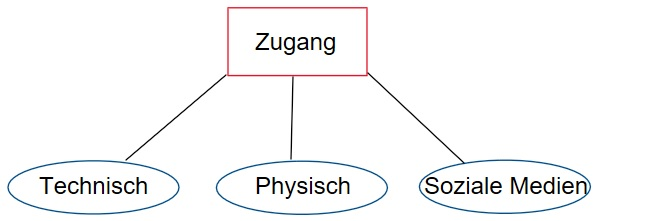
\includegraphics[width = 10cm]{figures/Zugang.jpg}
\caption{verschiedene Zugangsarten}
(eigene Darstellung)
\label{fig:verschiedene Zugangsarten}
\end{figure}

Social Engineering in seiner schädlichen Ausprägung lässt sich typischerweise in drei Hauptkategorien einteilen: Phishing, Elizitieren per Telefon und Identitätsbetrug (vgl. \cite{GrundformenDesSE})

\subsection{Phishing}

Phishing scams might be the most common types of social engineering attacks used
today. Most phishing scams tend to have the following characteristics (Bisson, 2015):
• They seek to obtain personally identifiable information (PII), such as names, addresses
and social security numbers.
• They tend to use shortened URLs or embed links that redirect users to sites that appear
legitimate.
• They usually attempt to instill a sense of urgency in the user by using some sort of fear
tactic or a threat in an attempt to get the user to act immediately.
Some phishing emails are more poorly crafted than others to the extent that their
messages oftentimes exhibit spelling and grammar errors but these emails are no less focused
on directing victims to a fake website or form where they can steal user login credentials and
other personal information (Workman, 2008).
A recent scam sent phishing emails to users after they installed cracked APK files from
Google Play Books that were pre-loaded with malware. This specific phishing campaign
demonstrates how attackers commonly pair malware with phishing attacks in an effort to steal
users’ information (Whitwam, 2015).

Die Form des „Phishing“ oder eben des Angelns nach Informationen ist die wohl am weitesten
verbreitete, vor allem durch den Versand von Massen-E-Mails oder durch zielgerichtete
E-Mails. In diesen E-Mails sind schädliche Dateien, Links oder Instruktionen für
den Adressaten enthalten. Die Konsequenzen durch eine Öffnung dieser Mails sind vielschichtig
und oft äußerst bedrohlich.
Ebenfalls unter die Kategorie des „Phishing“ fallen die zielgerichteten Angriffe auf
(hochrangige) Exponenten von Unternehmen. Wenn es sich um persönlich formulierte
E-Mails, die bereits Detailinformationen über den Adressaten beinhalten handelt, sprechen
wir von „Spear-Phishing“ – abgeleitet vom Speer, welcher sich fokussiert auf ein
Subjekt richtet.

In der Umgangssprache bekannt und in letzter Zeit eine immer häufiger angewendete
Form des Phishing ist der CEO-Fraud oder eben das „Whaling“ – abgeleitet vom Wal.
Dies umschreibt das Spear-Phishing auf ein hochrangiges Individuum. Die Schäden aus
diesen Whaling-Methoden sind enorm, und die Anzahl dieser Angriffe, auch „Business
E-mail Compromise (BEC)“ genannt, steigt rasant (Federal Bureau of Investigations 2016).
Das Internet Complaint Center des FBI hat im Jahr 2016 bereits über 22.000 Unternehmen
und Organisationen als Opfer dieser Betrugsform identifiziert. Die Dunkelziffer ist
auch bei diesen Taten hoch, und man kann davon ausgehen, dass nur ein geringer Prozentsatz
an Betroffenen an die Öffentlichkeit gelangt.
Die fünf häufigsten Betrugsmuster gemäß dieser Studie des FBI aus dem Jahr 2016
seien die folgenden (Federal Bureau of Investigations 2016):
1. Drittparteien: Unternehmen werden mit gefälschten angeblichen Lieferantenangaben
angeschrieben, Rechnungen an das vermeintliche Konto des Lieferanten – das auf die
Täter lautet – zu bezahlen. In der Praxis lässt sich dieses Muster häufig beobachten.
2. CEO-Fraud: Anhand kompromittierter E-Mail-Accounts auf Stufe C-Level wie CEO,
CFO, CTO, CSO, CIO (Geschäftsleitung/Vorstand) werden Mitarbeiter aufgefordert,
Geld an ein bestimmtes Konto zu überweisen oder überweisen zu lassen. Die
E-Mail-Konten können dabei gefälscht oder tatsächlich gehackt und übernommen worden
sein. Die hier angewandte Methode ist auch unter den Namen „Business Executive
Scam“ oder „Financial Industry Wire Frauds“ bekannt.
3. Datendiebstahl auf Basis CEO-Fraud: Gefälschte E-Mails auf Stufe C-Level werden
genutzt, um sensible Daten abzugreifen. Es kann sich dabei um Daten aus der Personalabteilung,
der Buchhaltung, des Controlling oder des Geschäftsleitungssekretariats
handeln.
4. Weitere betrügerische Kommunikation: Die persönlichen E-Mail-Accounts von Mitarbeitern
werden gehackt und zur Kommunikation mit Dritten (Geschäftspartnern,
Kunden, Lieferanten etc.) genutzt. Auch hier wird wieder um Zahlung von Beträgen an
die Konten der Täter gebeten.

\begin{figure}[h]
    \centering
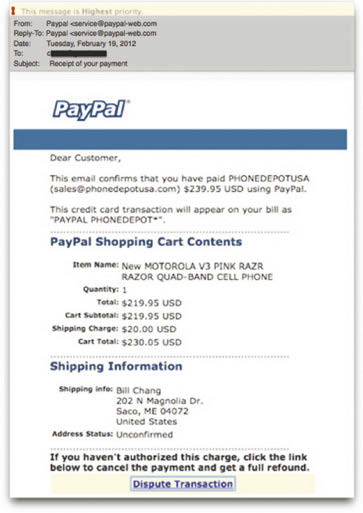
\includegraphics[width = 5cm]{figures/ChristopherHadn_2014_Kapitel2WasIstSocialE_SocialEngineeringEntt.jpg}
\caption{gefälschte E-Mail von PayPal}
\cite{GrundformenDesSE}
\label{fig:PhishingPayPal}
\end{figure}




\subsection{Elizitieren per Telefon}
\subsection{Identitätsbetrug}


\section{weitere Angriffsvektoren}

\subsection{Dumpster diving}
\subsection{Watering Hole}
\subsection{Ködern}
\subsection{Honigtopf}
\subsection{Tailgating/Piggybacking}


\section{Psychologische Prinzipien hinter Social Engineering}

\subsection{Mittel der Manipulation}

\subsection{Mittel der Beeinflussung}

\subsubsection{stereotypes Verhalten}
\subsubsection{Reziprozität}
\subsubsection{Verpflichtung und Konsistenz}
\subsubsection{Soziale Bewährtheit}
\subsubsection{Sympathie}
\subsubsection{Authorität}
\subsubsection{Knappheit}

%\section{Beispiel eines erfolgreichen Social Engineering Angriffs}
